% ============================================================
% HPTU Nueva Sede — Presentación Ejecutiva para Tomadores de Decisión
% Storytelling narrativo · 22 slides · ~25 minutos
% Compilar con: lualatex hptu-ejecutiva-6mar.tex
% ============================================================
\documentclass[aspectratio=169, 11pt]{beamer}

% ── Tema ────────────────────────────────────────────────────
\usetheme{default}
\usecolortheme{default}
\setbeamertemplate{navigation symbols}{}
\setbeamertemplate{footline}{%
  \hfill{\tiny\textcolor{slate!60}{\insertframenumber\,/\,\inserttotalframenumber}}\hspace{8pt}\vspace{4pt}%
}

% Paleta HPTU
\definecolor{hptu}{HTML}{00549F}
\definecolor{hptudark}{HTML}{003D75}
\definecolor{teal}{HTML}{0D9488}
\definecolor{coral}{HTML}{EF4444}
\definecolor{amber}{HTML}{F59E0B}
\definecolor{slate}{HTML}{64748B}
\definecolor{bglight}{HTML}{F8FAFC}
\definecolor{green}{HTML}{22C55E}
\definecolor{violet}{HTML}{8B5CF6}

\setbeamercolor{frametitle}{fg=hptu}
\setbeamercolor{title}{fg=white}
\setbeamercolor{subtitle}{fg=white!85}
\setbeamercolor{author}{fg=white!80}
\setbeamercolor{date}{fg=white!70}
\setbeamercolor{normal text}{fg=black!85}
\setbeamercolor{structure}{fg=hptu}
\setbeamercolor{itemize item}{fg=teal}
\setbeamercolor{itemize subitem}{fg=hptu}
\setbeamercolor{block title}{fg=white, bg=hptu}
\setbeamercolor{block body}{bg=bglight}
\setbeamercolor{block title alerted}{fg=white, bg=coral}
\setbeamercolor{block body alerted}{bg=coral!5}
\setbeamercolor{block title example}{fg=white, bg=teal}
\setbeamercolor{block body example}{bg=teal!5}

\setbeamerfont{frametitle}{size=\Large, series=\bfseries}
\setbeamerfont{title}{size=\Huge, series=\bfseries}
\setbeamerfont{subtitle}{size=\large}
\setbeamertemplate{itemize items}[circle]

% ── Paquetes ────────────────────────────────────────────────
\usepackage{fontspec}
\usepackage{booktabs}
\usepackage{tabularx}
\usepackage{colortbl}
\usepackage{graphicx}
\usepackage{tikz}
\usetikzlibrary{calc, positioning, shapes.geometric, arrows.meta, backgrounds}
\usepackage{pgfplots}
\pgfplotsset{compat=1.18}
\usepackage{multicol}
\usepackage{hyperref}

% Fuentes
\setsansfont{Helvetica Neue}[
  BoldFont={Helvetica Neue Bold},
  ItalicFont={Helvetica Neue Italic},
]

\newcommand{\highlight}[1]{\textcolor{teal}{\textbf{#1}}}
\newcommand{\danger}[1]{\textcolor{coral}{\textbf{#1}}}
\newcommand{\src}[1]{\par\vspace{2pt}{\tiny\textcolor{slate}{Fuente: #1}}}

% ── Metadata ────────────────────────────────────────────────
\title{Nueva Sede HPTU}
\subtitle{Estudio de Localización Estratégica\\[4pt]{\normalsize Avance Fases 1 y 2 — Conclusiones Preliminares}}
\author{Fourier.dev · Equipo de Análisis Estratégico}
\date{6 de marzo, 2026}

\begin{document}

% ============================================================
% SLIDE 1 — PORTADA
% ============================================================
{
\setbeamercolor{background canvas}{bg=hptu}
\begin{frame}[plain]
\vfill
\begin{center}
{\usebeamerfont{title}\usebeamercolor[fg]{title}\inserttitle}

\vspace{10pt}
{\usebeamerfont{subtitle}\usebeamercolor[fg]{subtitle}\insertsubtitle}

\vspace{22pt}
\begin{tikzpicture}
  \draw[white, line width=0.5pt] (0,0) -- (8,0);
\end{tikzpicture}

\vspace{14pt}
{\small\textcolor{white!80}{
3.8 millones de registros · 15 fuentes oficiales · Cero estimaciones}}

\vspace{6pt}
{\small\textcolor{white!60}{
5 zonas evaluadas · 12 capas interactivas · Modelo MCDA calibrado}}

\vspace{22pt}
{\footnotesize\textcolor{white!50}{\insertauthor}}

\vspace{4pt}
{\footnotesize\usebeamercolor[fg]{date}\insertdate}
\end{center}
\vfill
\end{frame}
}

% ============================================================
% SLIDE 2 — EL PROBLEMA
% ============================================================
{
\setbeamercolor{background canvas}{bg=coral!3}
\begin{frame}{El contexto: un hospital saturado, lejos de su mercado}

\begin{columns}[T]
\column{0.52\textwidth}
Hoy, el Hospital Pablo Tobón Uribe opera en Robledo con \textbf{1,094 camas}.
De esas, \danger{solo 44 están disponibles}.

\vspace{2pt}
\begin{center}
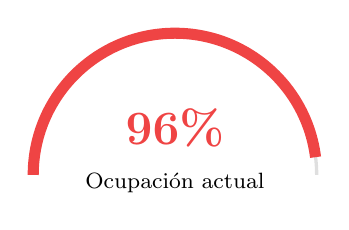
\begin{tikzpicture}
  \draw[gray!25, very thick] (0,0) arc (180:0:1.8);
  \draw[coral, line width=4pt] (0,0) arc (180:7.2:1.8);
  \node[font=\LARGE\bfseries, coral] at (1.8, 0.6) {96\%};
  \node[font=\footnotesize, below] at (1.8, 0.15) {Ocupación actual};
\end{tikzpicture}
\end{center}

\vspace{2pt}
{\small Mientras tanto, la población que más demanda servicios de alta complejidad ---estratos 5 y 6--- está en \textbf{El Poblado y el corredor Las Palmas}. A más de 20 minutos de Robledo.

\vspace{4pt}
Y ese corredor tiene \danger{exactamente cero camas} de alta complejidad.}

\column{0.45\textwidth}
\vspace{2pt}
\begin{alertblock}{\small El contexto regional}
\footnotesize
La OMS recomienda \textbf{3--5 camas} por 1,000 hab.

\vspace{3pt}
\begin{tabular}{@{}lcc@{}}
\toprule
\textbf{Municipio} & \textbf{Camas/1K} & \\
\midrule
\rowcolor{coral!10}
Medellín & \danger{1.0} & {\tiny $\times$3 del mínimo} \\
\rowcolor{coral!8}
Envigado & \danger{0.6} & {\tiny $\times$5 del mínimo} \\
Itagüí & \danger{0.6} & \\
Sabaneta & \danger{0.5} & \\
\midrule
\textbf{OMS mínimo} & \highlight{3.0} & \\
\bottomrule
\end{tabular}
\end{alertblock}

\vspace{4pt}
\begin{exampleblock}{\small La pregunta que guía este estudio}
\centering
\textbf{¿Dónde debería ubicarse la nueva sede?}
\end{exampleblock}
\end{columns}
\end{frame}
}

% ============================================================
% SLIDE 3 — METODOLOGÍA
% ============================================================
\begin{frame}{Dejamos que los datos hablen}

{\small Diseñamos un modelo de \textbf{Nodos y Flujos de Valor} en 4 fases. Hoy presentamos los hallazgos de las dos primeras, y un avance financiero preliminar.}

\vspace{10pt}
\begin{center}
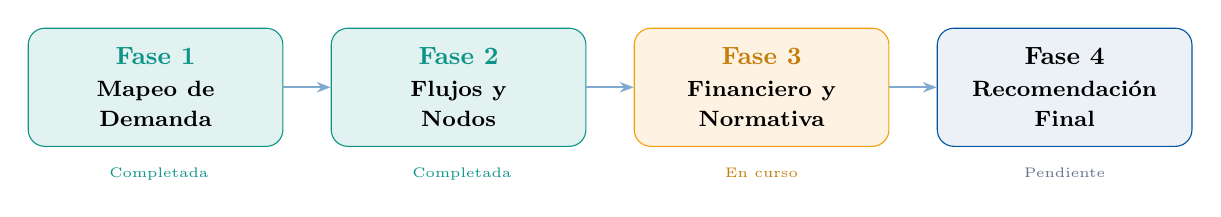
\begin{tikzpicture}[
  node distance=0.6cm,
  phase/.style={draw=hptu, fill=hptu!8, rounded corners=6pt,
                text width=3.0cm, minimum height=1.5cm, align=center,
                font=\small\bfseries},
  done/.style={phase, fill=teal!12, draw=teal},
  active/.style={phase, fill=amber!12, draw=amber},
  arrow/.style={-{Stealth[length=5pt]}, thick, hptu!50}
]
\node[done] (p1) {\textcolor{teal}{Fase 1}\\[2pt]\footnotesize Mapeo de\\Demanda};
\node[done, right=of p1] (p2) {\textcolor{teal}{Fase 2}\\[2pt]\footnotesize Flujos y\\Nodos};
\node[active, right=of p2] (p3) {\textcolor{amber!80!black}{Fase 3}\\[2pt]\footnotesize Financiero y\\Normativa};
\node[phase, right=of p3] (p4) {Fase 4\\[2pt]\footnotesize Recomendación\\Final};

\draw[arrow] (p1) -- (p2);
\draw[arrow] (p2) -- (p3);
\draw[arrow] (p3) -- (p4);

\node[below=4pt of p1, font=\tiny\color{teal}] {\checkmark\ Completada};
\node[below=4pt of p2, font=\tiny\color{teal}] {\checkmark\ Completada};
\node[below=4pt of p3, font=\tiny\color{amber!80!black}] {En curso};
\node[below=4pt of p4, font=\tiny\color{slate}] {Pendiente};
\end{tikzpicture}
\end{center}

\vspace{12pt}
{\small Cada zona candidata recibe un \textbf{score de 0 a 100} con cuatro dimensiones ponderadas:}

\vspace{8pt}
\begin{center}
{\large
$\text{Score} = \underbrace{A \times 35\%}_{\text{Accesibilidad}} + \underbrace{D \times 30\%}_{\text{Demanda}} + \underbrace{C \times 20\%}_{\text{Competencia}} + \underbrace{V \times 15\%}_{\text{Valor Inmob.}}$
}
\end{center}

\vspace{8pt}
{\small\textcolor{slate}{Todos los datos provienen de fuentes oficiales verificables. Cada número tiene trazabilidad a su dataset original.}}
\end{frame}

% ============================================================
% SLIDE 4 — LA BASE DE EVIDENCIA
% ============================================================
\begin{frame}{La base de evidencia: 15 fuentes, 3.8 millones de registros}

\vspace{2pt}
{\scriptsize
\begin{tabular}{@{}p{4.2cm}lrp{5.2cm}@{}}
\toprule
\textbf{Fuente} & \textbf{Dataset} & \textbf{Registros} & \textbf{Uso en el estudio} \\
\midrule
Catastro Municipal Medellín & bp59-rj8r & 1,041,413 & Predios por estrato, avalúos, barrio \\
DENSURBAM (URBAM/EAFIT) & densurbam.com.co & 1,220,415 & IRS salud, sostenibilidad, proy.\ 2037 \\
MEData Velocidades & 7t5n-3b3w & 682,502 & Velocidades por corredor 2017--2020 \\
POT Bat.\ Indicadores & 3ciz-tpgr & 331,741 & CL\_D, ICS, alturas, suelo potencial \\
Lotes Potenciales & m4wi-nn8x & 441,966 & 592 lotes en corredor Las Palmas \\
MEData Aforos & b9s9-jw7c & 74,900 & Volúmenes vehiculares por hora \\
Licencias Urbanísticas & pxmc-bbtu & 32,266 & 27 licencias dotacional/salud \\
REPS Prestadores & b4dp-ximh & 1,536 & IPS habilitadas, camas, complejidad \\
REPS Capacidad Inst.\ & s2ru-bqt6 & 1,711 & Camas por tipo, nov.\ 2022 \\
DANE CNPV 2018 & evm3-92yw & 465 & Población por municipio y edad \\
OSM Overpass API & Overpass QL & 1,323 & 178 salud, 750 educación, 330 comercio \\
Mapbox Matrix / Directions & API v1 & 40 & Tiempos reales, isocronas, rutas \\
Google Routes API & Routes v2 & 12 & Validación cruzada de tiempos \\
ArcGIS Estratos & FeatureServer & 5,142 & Manzanas censales por estrato \\
EPM Cobertura & datos.gov.co & 951 & Suscriptores E6 por comuna \\
\bottomrule
\end{tabular}
}

\vspace{8pt}
\begin{center}
{\small\textbf{Total: 3,836,383 registros} de fuentes oficiales verificables. Cero datos estimados.\\[2pt]
Cada métrica presentada hoy tiene trazabilidad completa a su dataset de origen.}
\end{center}
\end{frame}

% ============================================================
% SLIDE 5 — ARQUITECTURA DE DATOS (NUEVO)
% ============================================================
{
\setbeamercolor{background canvas}{bg=hptu!3}
\begin{frame}{Del registro crudo a la decisión: arquitectura de datos}

{\small Construimos un pipeline reproducible. Cada dato presentado hoy puede rastrearse hasta su fuente original.}

\vspace{8pt}
\begin{center}
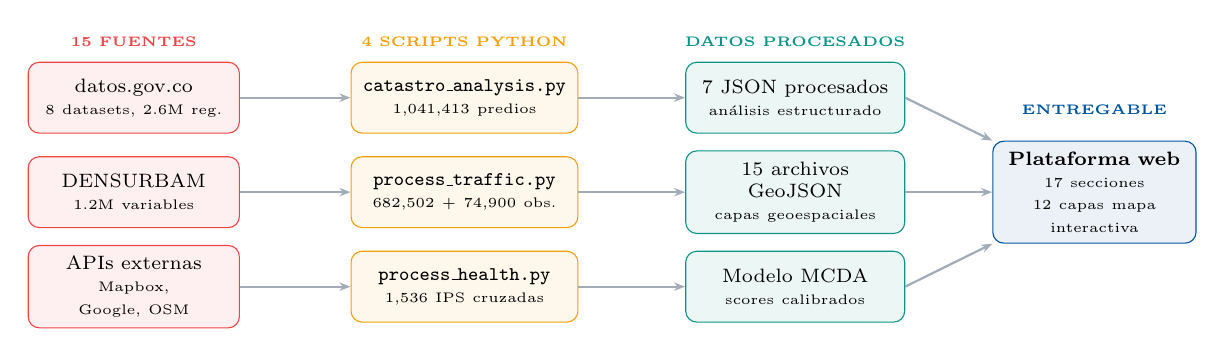
\begin{tikzpicture}[
  bx/.style={rounded corners=4pt, minimum height=0.9cm,
             align=center, font=\scriptsize, inner sep=4pt},
  arr/.style={-{Stealth[length=4pt]}, thick, slate!60},
]
% Column 1: Sources
\node[bx, draw=coral, fill=coral!8, text width=2.4cm] (s1) at (0, 2.0) {datos.gov.co\\{\tiny 8 datasets, 2.6M reg.}};
\node[bx, draw=coral, fill=coral!8, text width=2.4cm] (s2) at (0, 0.8) {DENSURBAM\\{\tiny 1.2M variables}};
\node[bx, draw=coral, fill=coral!8, text width=2.4cm] (s3) at (0,-0.4) {APIs externas\\{\tiny Mapbox, Google, OSM}};

% Column 2: Scripts
\node[bx, draw=amber, fill=amber!8, text width=2.6cm] (p1) at (4.2, 2.0) {\texttt{catastro\_analysis.py}\\{\tiny 1,041,413 predios}};
\node[bx, draw=amber, fill=amber!8, text width=2.6cm] (p2) at (4.2, 0.8) {\texttt{process\_traffic.py}\\{\tiny 682,502 + 74,900 obs.}};
\node[bx, draw=amber, fill=amber!8, text width=2.6cm] (p3) at (4.2,-0.4) {\texttt{process\_health.py}\\{\tiny 1,536 IPS cruzadas}};

% Column 3: Outputs
\node[bx, draw=teal, fill=teal!8, text width=2.5cm] (o1) at (8.4, 2.0) {7 JSON procesados\\{\tiny análisis estructurado}};
\node[bx, draw=teal, fill=teal!8, text width=2.5cm] (o2) at (8.4, 0.8) {15 archivos GeoJSON\\{\tiny capas geoespaciales}};
\node[bx, draw=teal, fill=teal!8, text width=2.5cm] (o3) at (8.4,-0.4) {Modelo MCDA\\{\tiny scores calibrados}};

% Column 4: Platform
\node[bx, draw=hptu, fill=hptu!8, text width=2.3cm] (w1) at (12.2, 0.8) {\textbf{Plataforma web}\\{\tiny 17 secciones}\\{\tiny 12 capas mapa}\\{\tiny interactiva}};

% Arrows
\draw[arr] (s1) -- (p1); \draw[arr] (p1) -- (o1);
\draw[arr] (s2) -- (p2); \draw[arr] (p2) -- (o2);
\draw[arr] (s3) -- (p3); \draw[arr] (p3) -- (o3);
\draw[arr] (o1.east) -- (w1.north west);
\draw[arr] (o2.east) -- (w1.west);
\draw[arr] (o3.east) -- (w1.south west);

% Labels
\node[font=\tiny\bfseries, coral, above=2pt of s1] {15 FUENTES};
\node[font=\tiny\bfseries, amber, above=2pt of p1] {4 SCRIPTS PYTHON};
\node[font=\tiny\bfseries, teal, above=2pt of o1] {DATOS PROCESADOS};
\node[font=\tiny\bfseries, hptu, above=6pt of w1] {ENTREGABLE};

\end{tikzpicture}
\end{center}

\vspace{6pt}
\begin{columns}[T]
\column{0.48\textwidth}
\begin{block}{\small Reproducibilidad}
\scriptsize Cada script está versionado. Los datasets tienen ID único (ej: \texttt{bp59-rj8r}). Cualquier métrica puede verificarse ejecutando el pipeline desde cero.
\end{block}
\column{0.48\textwidth}
\begin{block}{\small Validación cruzada}
\scriptsize Tiempos de viaje validados con 2 APIs independientes (Mapbox + Google Routes). Ubicaciones de IPS cruzadas con REPS + OSM + Google Geocoding.
\end{block}
\end{columns}

\end{frame}
}

% ============================================================
% SLIDE 6 — EL MERCADO OBJETIVO
% ============================================================
\begin{frame}{¿A quién va dirigida la nueva sede?}

\begin{columns}[T]
\column{0.50\textwidth}
{\small Analizamos \textbf{1,041,413 predios} del Catastro Municipal.
El mercado objetivo está concentrado y es cuantificable.}

\vspace{4pt}
{\scriptsize
\begin{tabular}{@{}lrrc@{}}
\toprule
\textbf{Barrio} & \textbf{E5/E6} & \textbf{\%} & \textbf{Avalúo} \\
\midrule
\rowcolor{teal!8}
\textbf{El Poblado core} & \textbf{38,415} & \textbf{98\%} & \$371M \\
Castropol & 6,228 & 97\% & \$327M \\
Los Balsos No.\ 1 & 4,019 & 95\% & \$401M \\
San Lucas & 3,671 & 93\% & \$512M \\
\rowcolor{teal!6}
Altos del Poblado & 1,867 & 91\% & \$245M \\
El Tesoro & 1,856 & 89\% & \$258M \\
Los Balsos No.\ 2 & 2,143 & 88\% & \$347M \\
{\tiny + 15 barrios más} & & & \\
\midrule
\textbf{Total 22 barrios} & \textbf{174,543} & & \\
\bottomrule
\end{tabular}
}

\vspace{2pt}
\src{Catastro Municipal Medellín (bp59-rj8r), 1,041,413 predios}

\column{0.47\textwidth}
\vspace{2pt}
\begin{exampleblock}{\small El ecosistema del corredor}
\footnotesize
No son solo predios. Es un \textbf{ecosistema} de alta capacidad de pago:

\vspace{3pt}
\begin{itemize}\setlength{\itemsep}{1pt}
  \item \textbf{Prepagada}: SURA Salud El Poblado, \highlight{320K afiliados}
  \item \textbf{30 colegios premium}: Colombo Británico, Montessori, Columbus --- familias E5/E6
  \item \textbf{Clubes}: El Rodeo, Campestre --- red de referidos
  \item \textbf{Corporativo}: Milla de Oro, Bancolombia HQ (4K empleados con prepagada)
\end{itemize}
\end{exampleblock}

\vspace{2pt}
\begin{alertblock}{\small En resumen}
\scriptsize \highlight{174K predios} E5/E6 en 22 barrios (\textbf{\$245M--\$512M COP}). Ningún hospital cercano ofrece trasplantes u oncología compleja.
\end{alertblock}
\end{columns}
\end{frame}

% ============================================================
% SLIDE 7 — GRADIENTE DE DEMANDA (NUEVO)
% ============================================================
\begin{frame}{El gradiente de demanda a lo largo del corredor}

{\small La demanda no se distribuye uniformemente. Se concentra en la parte baja del corredor y \textbf{cae drásticamente} al subir por Las Palmas.}

\vspace{4pt}
\begin{center}
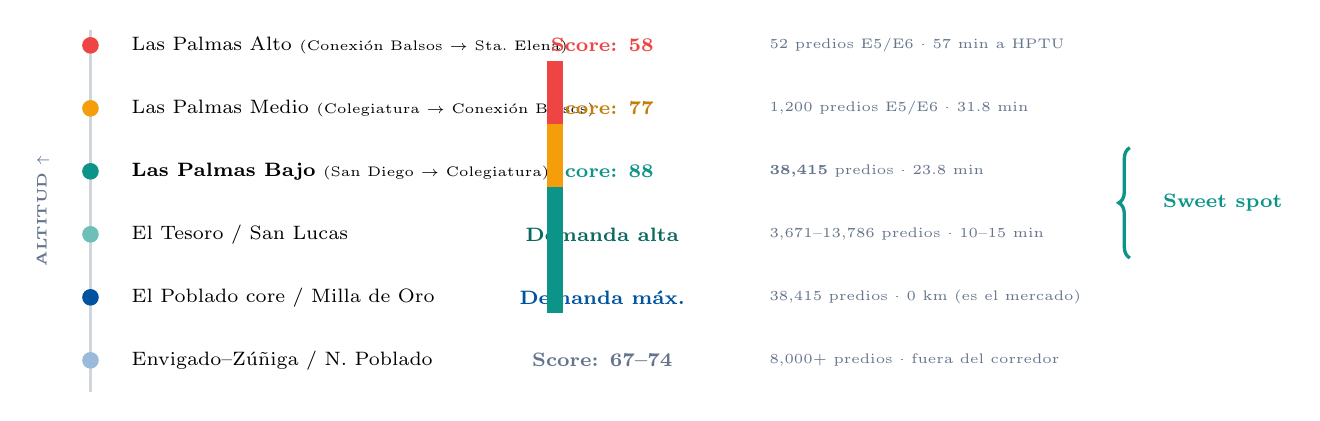
\begin{tikzpicture}
% Vertical axis (altitude metaphor)
\draw[slate!30, thick] (0, 0) -- (0, -4.6);
\node[font=\tiny\bfseries, slate, rotate=90, anchor=south] at (-0.4, -2.3) {ALTITUD $\uparrow$};

% Points along corridor — compressed vertical spacing
\fill[coral] (0, -0.2) circle (3pt);
\node[font=\scriptsize, anchor=west] at (0.4, -0.2) {Las Palmas Alto {\tiny(Conexión Balsos $\rightarrow$ Sta.\ Elena)}};
\node[font=\scriptsize\bfseries, coral] at (6.5, -0.2) {Score: 58};
\node[font=\tiny, slate, anchor=west] at (8.5, -0.2) {52 predios E5/E6 · 57 min a HPTU};

\fill[amber] (0, -1.0) circle (3pt);
\node[font=\scriptsize, anchor=west] at (0.4, -1.0) {Las Palmas Medio {\tiny(Colegiatura $\rightarrow$ Conexión Balsos)}};
\node[font=\scriptsize\bfseries, amber!80!black] at (6.5, -1.0) {Score: 77};
\node[font=\tiny, slate, anchor=west] at (8.5, -1.0) {1,200 predios E5/E6 · 31.8 min};

\fill[teal] (0, -1.8) circle (3pt);
\node[font=\scriptsize, anchor=west] at (0.4, -1.8) {\textbf{Las Palmas Bajo} {\tiny(San Diego $\rightarrow$ Colegiatura)}};
\node[font=\scriptsize\bfseries, teal] at (6.5, -1.8) {Score: 88};
\node[font=\tiny, slate, anchor=west] at (8.5, -1.8) {\textbf{38,415} predios · 23.8 min};

\fill[teal!60] (0, -2.6) circle (3pt);
\node[font=\scriptsize, anchor=west] at (0.4, -2.6) {El Tesoro / San Lucas};
\node[font=\scriptsize\bfseries, teal!70!black] at (6.5, -2.6) {Demanda alta};
\node[font=\tiny, slate, anchor=west] at (8.5, -2.6) {3,671--13,786 predios · 10--15 min};

\fill[hptu] (0, -3.4) circle (3pt);
\node[font=\scriptsize, anchor=west] at (0.4, -3.4) {El Poblado core / Milla de Oro};
\node[font=\scriptsize\bfseries, hptu] at (6.5, -3.4) {Demanda máx.};
\node[font=\tiny, slate, anchor=west] at (8.5, -3.4) {38,415 predios · 0 km (es el mercado)};

\fill[hptu!40] (0, -4.2) circle (3pt);
\node[font=\scriptsize, anchor=west] at (0.4, -4.2) {Envigado--Zúñiga / N.\ Poblado};
\node[font=\scriptsize\bfseries, slate] at (6.5, -4.2) {Score: 67--74};
\node[font=\tiny, slate, anchor=west] at (8.5, -4.2) {8,000+ predios · fuera del corredor};

% Gradient bar
\fill[teal] (5.8, -2.0) rectangle (6.0, -3.6);
\fill[amber] (5.8, -1.2) rectangle (6.0, -2.0);
\fill[coral] (5.8, -0.4) rectangle (6.0, -1.2);

% Bracket for sweet spot
\draw[teal, very thick, decorate, decoration={brace, amplitude=4pt, mirror}] (13.2, -1.5) -- (13.2, -2.9);
\node[font=\scriptsize\bfseries, teal, anchor=west] at (13.5, -2.2) {Sweet spot};

\end{tikzpicture}
\end{center}

\vspace{2pt}
{\small\textbf{Lectura clave}: La zona óptima está donde la demanda aún es alta pero el corredor ya fluye. Eso es Las Palmas Bajo ---desde San Diego hasta La Colegiatura--- donde convergen \highlight{38,415 predios E5/E6} con una vía a \highlight{40.9 km/h}.}

\end{frame}

% ============================================================
% SLIDE 8 — LA BRECHA HOSPITALARIA
% ============================================================
{
\setbeamercolor{background canvas}{bg=coral!3}
\begin{frame}{Un corredor sin hospital de alta complejidad}

\begin{columns}[T]
\column{0.48\textwidth}
{\small Mapeamos \textbf{145 IPS} en el Valle de Aburrá. Esto es lo que encontramos:}

\vspace{4pt}
{\scriptsize
\begin{tabular}{@{}lrcl@{}}
\toprule
\textbf{Hospital} & \textbf{Camas} & \textbf{Ocup.} & \textbf{Dist. corredor} \\
\midrule
\rowcolor{coral!10}
HPTU Robledo & 1,094 & \danger{96\%} & 8.5 km \\
Cl.\ Medellín & 624 & 88\% & 3.2 km \\
\rowcolor{coral!6}
HGM ESE & 384 & \danger{92\%} & 7+ km \\
Cl.\ del Prado & 304 & 85\% & 5+ km \\
Cl.\ CES$^*$ & 213 & 82\% & \danger{7.16 km} \\
\midrule
\textbf{Total sistema} & \textbf{2,739} & \textbf{91\%} & \\
\bottomrule
\end{tabular}
}

\vspace{2pt}
{\scriptsize $^*$Verificada vía Google Geocoding: está en \textbf{Prado Centro}, no en Las Palmas.}
\src{REPS MinSalud (b4dp-ximh), Capacidad Instalada (s2ru-bqt6)}

\vspace{3pt}
\begin{block}{\small En el corredor Las Palmas}
\scriptsize
Cl.\ Rosario Tesoro (158 camas) y Cl.\ Las Vegas (171). Ninguna ofrece trasplantes ni oncología. Camas de alta complejidad: \danger{cero}.
\end{block}

\column{0.49\textwidth}
{\small\textbf{DENSURBAM confirma el déficit}} {\scriptsize(Var.\ 49 --- equipamiento salud):}

\vspace{2pt}
\begin{center}
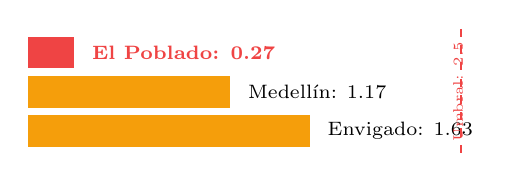
\begin{tikzpicture}
  \fill[coral] (0,0) rectangle (0.27/2.5*5.5, 0.4);
  \node[right, font=\scriptsize\bfseries] at (0.27/2.5*5.5+0.1, 0.2) {\danger{El Poblado: 0.27}};

  \fill[amber] (0,-0.5) rectangle (1.17/2.5*5.5, -0.1);
  \node[right, font=\scriptsize] at (1.17/2.5*5.5+0.1, -0.3) {Medellín: 1.17};

  \fill[amber] (0,-1.0) rectangle (1.63/2.5*5.5, -0.6);
  \node[right, font=\scriptsize] at (1.63/2.5*5.5+0.1, -0.8) {Envigado: 1.63};

  \draw[coral, thick, dashed] (2.5/2.5*5.5, 0.5) -- (2.5/2.5*5.5, -1.15);
  \node[font=\tiny, coral, rotate=90, anchor=south] at (2.5/2.5*5.5+0.15, -0.3) {Umbral: 2.5};
\end{tikzpicture}
\end{center}

\vspace{1pt}
{\tiny IRS = m² equipamiento / hab. DENSURBAM, URBAM-EAFIT / AMVA.}

\vspace{3pt}
{\small\textbf{10 barrios} del corredor: \danger{0.0 m²} de oferta de salud.}

\vspace{2pt}
{\scriptsize
\begin{tabular}{@{}lr@{}}
Población sin cobertura 2037 & \danger{103,913 hab.} \\
Infraestructura requerida & \danger{363,696 m²} \\
Crecimiento área focal & \highlight{+152,000 personas} \\
\end{tabular}
}

\vspace{3pt}
{\scriptsize No es solo oportunidad de mercado. Es \textbf{necesidad de infraestructura}.}
\end{columns}
\end{frame}
}

% ============================================================
% SLIDE 9 — PROYECCIÓN 2037: DÉFICIT CRECIENTE (NUEVO)
% ============================================================
{
\setbeamercolor{background canvas}{bg=coral!3}
\begin{frame}{Proyección 2037: un déficit que crece}

{\small DENSURBAM (URBAM/EAFIT) modela 59 variables de sostenibilidad territorial con \textbf{1,220,415 registros}. La variable 49 mide equipamiento de salud en m²/habitante.}

\vspace{6pt}
\begin{columns}[T]
\column{0.52\textwidth}

{\scriptsize
\begin{tabular}{@{}p{3.0cm}ccr@{}}
\toprule
\textbf{Barrio} & \textbf{Oferta} & \textbf{Déficit} & \textbf{Pob.\ 2037} \\
 & {\tiny m²/hab} & & \\
\midrule
\rowcolor{coral!10}
Altos del Poblado & \danger{0.0} & \danger{100\%} & 8,241 \\
\rowcolor{coral!10}
El Tesoro & \danger{0.0} & \danger{100\%} & 13,786 \\
\rowcolor{coral!10}
Los Balsos No.\ 1 & \danger{0.0} & \danger{100\%} & 13,484 \\
\rowcolor{coral!10}
Los Balsos No.\ 2 & \danger{0.0} & \danger{100\%} & 7,892 \\
\rowcolor{coral!8}
San Lucas & \danger{0.0} & \danger{100\%} & 9,312 \\
\rowcolor{coral!8}
La Florida & \danger{0.0} & \danger{100\%} & 15,570 \\
\rowcolor{coral!8}
Alejandría & \danger{0.0} & \danger{100\%} & 8,728 \\
\rowcolor{coral!6}
Castropol & \danger{0.0} & \danger{100\%} & 14,303 \\
\rowcolor{coral!6}
La Aguacatala & \danger{0.0} & \danger{100\%} & 6,521 \\
\rowcolor{coral!6}
El Diamante II & \danger{0.0} & \danger{100\%} & 6,076 \\
\midrule
\textbf{Total 10 barrios} & \danger{0.0} & \danger{100\%} & \textbf{103,913} \\
\bottomrule
\end{tabular}
}

\src{DENSURBAM (densurbam.com.co), 1,220,415 registros, proy.\ 2037}

\column{0.45\textwidth}
\begin{alertblock}{\small Las cifras del déficit}
\footnotesize
\begin{tabular}{@{}lr@{}}
Demanda m²/hab (estándar) & 3.5 \\
Oferta actual corredor & \danger{0.0} \\
Déficit & \danger{100\%} \\
\midrule
Población 2037 & 103,913 \\
m² requeridos & \danger{363,696} \\
\end{tabular}
\end{alertblock}

\vspace{4pt}
\begin{block}{\small Crecimiento poblacional}
\scriptsize
Proyecciones DENSURBAM al 2037:

\vspace{2pt}
\begin{tabular}{@{}lr@{}}
Medellín & +6.1\% \\
Envigado & +17.1\% \\
Sabaneta & +20.6\% \\
\textbf{Área focal} & \highlight{+152,000 hab.} \\
\end{tabular}

\vspace{3pt}
El corredor crece, pero la oferta de salud de alta complejidad sigue en \danger{cero}.
\end{block}

\end{columns}
\end{frame}
}

% ============================================================
% SLIDE 10 — EL TRÁFICO
% ============================================================
\begin{frame}{¿Se puede llegar? Los datos de movilidad responden}

\begin{columns}[T]
\column{0.50\textwidth}
Procesamos \highlight{682,502 observaciones} de velocidad de la plataforma MEData (2017--2020):

\vspace{4pt}
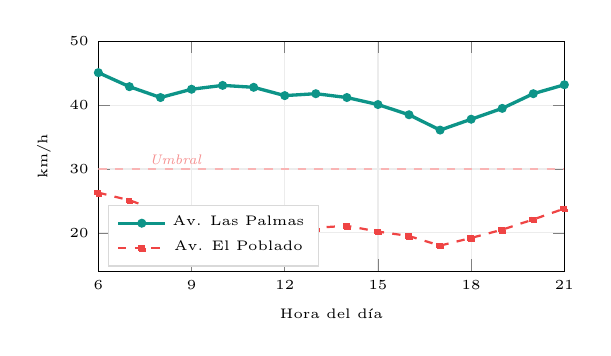
\begin{tikzpicture}
\begin{axis}[
  width=7.5cm, height=4.5cm,
  xlabel={\tiny Hora del día},
  ylabel={\tiny km/h},
  xmin=6, xmax=21, ymin=14, ymax=50,
  xtick={6,9,12,15,18,21},
  xticklabel style={font=\tiny},
  yticklabel style={font=\tiny},
  grid=major, grid style={gray!15},
  legend style={at={(0.02,0.02)}, anchor=south west, font=\tiny,
               fill=white, draw=gray!30},
]
\addplot[teal, very thick, mark=*, mark size=1pt] coordinates {
  (6,45.1)(7,42.9)(8,41.2)(9,42.5)(10,43.1)(11,42.8)
  (12,41.5)(13,41.8)(14,41.2)(15,40.1)(16,38.5)(17,36.1)
  (18,37.8)(19,39.5)(20,41.8)(21,43.2)
};
\addlegendentry{Av. Las Palmas}
\addplot[coral, thick, dashed, mark=square*, mark size=1pt] coordinates {
  (6,26.3)(7,25.1)(8,23.4)(9,22.8)(10,21.9)(11,21.2)
  (12,20.5)(13,20.8)(14,21.1)(15,20.2)(16,19.5)(17,18.0)
  (18,19.2)(19,20.5)(20,22.1)(21,23.8)
};
\addlegendentry{Av. El Poblado}
\addplot[coral!40, thin, dashed] coordinates {(6,30)(21,30)};
\node[font=\tiny, coral!60] at (axis cs:8.5,31.5) {\textit{Umbral}};
\end{axis}
\end{tikzpicture}

\src{MEData Vel.\ Tiempo Viaje GT (7t5n-3b3w), 682K obs.}

\column{0.47\textwidth}
\vspace{4pt}
A las \textbf{5:00 PM} ---la peor hora---:

\vspace{3pt}
\begin{alertblock}{}
\centering
{\Large \danger{18.0 km/h}}\\
\footnotesize Av.\ El Poblado — congestión severa
\end{alertblock}

\vspace{1pt}
\begin{exampleblock}{}
\centering
{\Large \highlight{36.1 km/h}}\\
\footnotesize Av.\ Las Palmas — \textbf{el doble de rápido}
\end{exampleblock}

\vspace{4pt}
{\footnotesize\textbf{Tiempos reales a la zona candidata:}}

\vspace{2pt}
{\scriptsize
\begin{tabular}{@{}lrl@{}}
Milla de Oro & \highlight{15.4 min} & Google Routes \\
El Poblado (Parque) & \highlight{17.7 min} & Google Routes \\
Envigado Centro & 24.8 min & Google Routes \\
Laureles & 32.3 min & Mapbox \\
Itagüí Centro & 33.4 min & Mapbox \\
\midrule
\textbf{Promedio} & \textbf{24.7 min} & \\
\end{tabular}
}

\vspace{2pt}
{\scriptsize El \textbf{80\%} del mercado E5/E6 llega en menos de 25 min.}
\end{columns}
\end{frame}

% ============================================================
% SLIDE 11 — COMPOSICIÓN VEHICULAR Y PATRONES (NUEVO)
% ============================================================
\begin{frame}{79,885 vehículos en un punto: composición y patrones}

{\small Además de velocidades, procesamos \textbf{74,900 registros de aforos} vehiculares. El Nodo 183 (Cra 43A $\times$ Calle 19) es el punto de entrada al corredor.}

\vspace{6pt}
\begin{columns}[T]
\column{0.45\textwidth}

\begin{center}
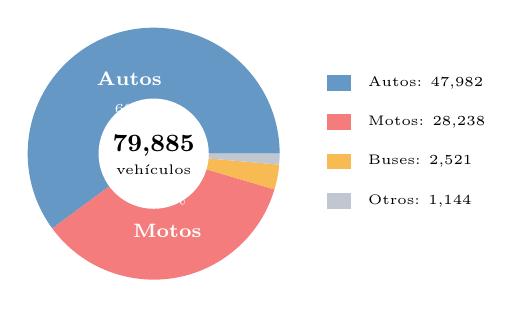
\begin{tikzpicture}
% Autos slice (60.1% = 216.4 degrees)
\fill[hptu!60] (0,0) -- (0:1.6) arc (0:216.4:1.6) -- cycle;
\node[font=\scriptsize\bfseries, white] at (108:1.0) {Autos};
\node[font=\tiny, white] at (108:0.6) {60.1\%};

% Motos slice (35.3% = 127.1 degrees)
\fill[coral!70] (0,0) -- (216.4:1.6) arc (216.4:343.5:1.6) -- cycle;
\node[font=\scriptsize\bfseries, white] at (280:1.0) {Motos};
\node[font=\tiny, white] at (280:0.6) {35.3\%};

% Buses + otros slices
\fill[amber!70] (0,0) -- (343.5:1.6) arc (343.5:355:1.6) -- cycle;
\fill[slate!40] (0,0) -- (355:1.6) arc (355:360:1.6) -- cycle;

% Center donut hole
\fill[white] (0,0) circle (0.7);
\node[font=\small\bfseries] at (0, 0.1) {79,885};
\node[font=\tiny] at (0, -0.2) {vehículos};

% Legend
\fill[hptu!60] (2.2, 0.8) rectangle (2.5, 1.0); \node[font=\tiny, right] at (2.6, 0.9) {Autos: 47,982};
\fill[coral!70] (2.2, 0.3) rectangle (2.5, 0.5); \node[font=\tiny, right] at (2.6, 0.4) {Motos: 28,238};
\fill[amber!70] (2.2,-0.2) rectangle (2.5, 0.0); \node[font=\tiny, right] at (2.6,-0.1) {Buses: 2,521};
\fill[slate!40] (2.2,-0.7) rectangle (2.5,-0.5); \node[font=\tiny, right] at (2.6,-0.6) {Otros: 1,144};
\end{tikzpicture}
\end{center}

\src{MEData Aforos Vehiculares (b9s9-jw7c), 74,900 registros}

\column{0.52\textwidth}

\begin{alertblock}{\small Patrones de pico}
\scriptsize
\begin{tabular}{@{}lrr@{}}
\toprule
\textbf{Período} & \textbf{Vehículos} & \textbf{\% del día} \\
\midrule
\rowcolor{amber!10}
AM Peak (6--8h) & 80,974 & 22.6\% \\
\rowcolor{coral!10}
\textbf{PM Peak (16--18h)} & \danger{95,145} & \danger{26.6\%} \\
Valle (10--15h) & 121,981 & 34.1\% \\
\midrule
\textbf{Total diario} & \textbf{358,100} & 100\% \\
\bottomrule
\end{tabular}

\vspace{3pt}
Hora pico absoluta: \danger{5:00 PM} (6,373 vehículos en 60 min).
\end{alertblock}

\vspace{3pt}
\begin{exampleblock}{\small Implicación para diseño}
\scriptsize
\begin{itemize}\setlength{\itemsep}{0pt}
  \item \textbf{35\% motos}: bahías de emergencia deben contemplar motociclistas
  \item \textbf{PM > AM}: urgencias nocturnas tienen mejor acceso vial
  \item \textbf{Ubicación post-cuello}: tráfico ya se ha filtrado al llegar a la zona candidata
\end{itemize}
\end{exampleblock}
\end{columns}

\end{frame}

% ============================================================
% SLIDE 12 — VIABILIDAD NORMATIVA POT (NUEVO)
% ============================================================
\begin{frame}{22 barrios evaluados: viabilidad normativa POT}

{\small Cruzamos \textbf{331,741 registros} de la Batería de Indicadores POT para evaluar qué barrios permiten uso dotacional de salud.}

\vspace{6pt}
{\scriptsize
\begin{tabular}{@{}p{3.2cm}ccrccl@{}}
\toprule
\textbf{Barrio} & \textbf{CL\_D} & \textbf{Alt.\ máx} & \textbf{Suelo pot.} & \textbf{ICS} & \textbf{Viabilidad} \\
\midrule
\rowcolor{teal!10}
\textbf{Altos del Poblado} & \textbf{2.38} & \textbf{11.7 p} & \textbf{68,020 m²} & 0.85 & \highlight{ALTA} \\
\rowcolor{teal!8}
Villa Carlota & 2.15 & 15.0 p & 171,198 m² & 0.78 & \highlight{ALTA} \\
\rowcolor{teal!8}
Barrio Colombia & 2.10 & 20.0 p & 90,905 m² & 0.82 & \highlight{ALTA} \\
\rowcolor{teal!6}
El Tesoro & 1.95 & 11.7 p & 45,200 m² & 0.80 & \highlight{ALTA} \\
\rowcolor{teal!6}
Castropol & 1.82 & 12.0 p & 38,500 m² & 0.76 & ALTA \\
Los Balsos No.\ 1 & 1.65 & 10.0 p & 22,800 m² & 0.72 & MEDIA-ALTA \\
San Lucas & 1.58 & 8.0 p & 15,600 m² & 0.70 & MEDIA-ALTA \\
La Florida & 1.42 & 6.0 p & 12,300 m² & 0.65 & MEDIA \\
Alejandría & 1.35 & 5.0 p & 8,900 m² & 0.60 & MEDIA \\
\rowcolor{coral!6}
Las Palmas Alto & 0.45 & 3.0 p & 5,200 m² & 0.30 & \danger{BAJA} \\
\bottomrule
\end{tabular}
}

\vspace{6pt}
\begin{columns}[T]
\column{0.48\textwidth}
\begin{block}{\small Qué significan estos indicadores}
\scriptsize
\begin{tabular}{@{}ll@{}}
\textbf{CL\_D} & Carga dotacional localizada \\
\textbf{Alt.\ máx} & Pisos permitidos por el POT \\
\textbf{Suelo pot.} & m² desarrollables disponibles \\
\textbf{ICS} & Índice de Construcción Social \\
\end{tabular}
\end{block}
\column{0.48\textwidth}
\begin{exampleblock}{\small Lectura clave}
\scriptsize \textbf{Altos del Poblado} tiene el CL\_D más alto del corredor (2.38), lo que indica que el POT \textbf{ya prevé} concentración de equipamiento dotacional en esa zona. No estamos forzando el uso del suelo: el territorio lo permite.
\end{exampleblock}
\end{columns}

\src{POT Batería de Indicadores (3ciz-tpgr), 331,741 registros. Lotes Potenciales (m4wi-nn8x), 441,966 registros.}
\end{frame}

% ============================================================
% SLIDE 13 — EL RANKING: 5 ZONAS
% ============================================================
\begin{frame}{Evaluamos cinco zonas con los mismos criterios}

{\small Aplicamos el modelo MCDA a \textbf{5 zonas candidatas}. Estos son los resultados:}

\vspace{8pt}
\begin{center}
{\small
\begin{tabular}{@{}lccccccr@{}}
\toprule
\textbf{Zona candidata} & \textbf{Acc.} & \textbf{Dem.} & \textbf{Comp.} & \textbf{Val.} & \textbf{SCORE} & \textbf{min HPTU} & \textbf{POT} \\
 & {\tiny 35\%} & {\tiny 30\%} & {\tiny 20\%} & {\tiny 15\%} & & & \\
\midrule
\rowcolor{teal!12}
\textbf{Las Palmas Bajo} & \textbf{92} & \textbf{93} & \textbf{78} & \textbf{80} & \highlight{88} & 23.8 & 9/9 \\
Las Palmas Medio & 72 & 84 & 82 & 70 & 77 & 31.8 & 6/9 \\
Envigado--Zúñiga & 75 & 80 & 62 & 74 & 74 & 22.4 & --- \\
N.\ Poblado--Itagüí & 82 & 68 & 52 & 58 & 67 & 19.0 & --- \\
\rowcolor{coral!6}
Las Palmas Alto & 42 & 52 & 90 & 62 & 58 & \danger{57.1} & N/A \\
\bottomrule
\end{tabular}
}
\end{center}

\vspace{8pt}
\begin{columns}[T]
\column{0.32\textwidth}
\begin{exampleblock}{\small \#1 Las Palmas Bajo: 88}
\footnotesize La \textbf{única zona} con score $>$80 en las \textbf{4 dimensiones}. Equilibrio entre cercanía al mercado, accesibilidad, y viabilidad normativa.
\end{exampleblock}

\column{0.32\textwidth}
\begin{block}{\small \#2 Las Palmas Medio: 77}
\footnotesize Pierde \textbf{11 puntos} por accesibilidad: 8 min más a HPTU y menor concentración de demanda. Más suelo disponible (132K m²).
\end{block}

\column{0.32\textwidth}
\begin{alertblock}{\small \#5 Las Palmas Alto: 58}
\footnotesize \danger{Descartado}. 57 min a HPTU, aislamiento geográfico, suelo rural. Inviable operativa y financieramente.
\end{alertblock}
\end{columns}
\end{frame}

% ============================================================
% SLIDE 14 — ISOCRONAS DE ACCESIBILIDAD (NUEVO)
% ============================================================
\begin{frame}{Isocronas: quién llega en 15, 20 y 30 minutos}

{\small Generamos isocronas reales con \textbf{Mapbox Isochrone API} para cada zona candidata, validadas con \textbf{Google Routes}.}

\vspace{6pt}
\begin{center}
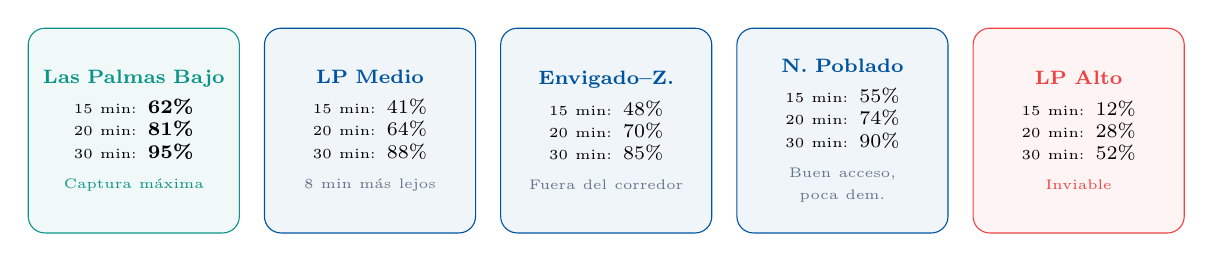
\begin{tikzpicture}[
  zn/.style={rounded corners=6pt, text width=2.4cm, minimum height=2.6cm,
             align=center, font=\scriptsize, inner sep=4pt},
]

\node[zn, draw=teal, fill=teal!6] (z1) at (0,0) {
  {\scriptsize\bfseries\textcolor{teal}{Las Palmas Bajo}}\\[3pt]
  {\tiny 15 min:} \textbf{62\%}\\
  {\tiny 20 min:} \textbf{81\%}\\
  {\tiny 30 min:} \textbf{95\%}\\[3pt]
  {\tiny\textcolor{teal}{Captura máxima}}
};

\node[zn, draw=hptu, fill=hptu!6] (z2) at (3.0,0) {
  {\scriptsize\bfseries\textcolor{hptu}{LP Medio}}\\[3pt]
  {\tiny 15 min:} 41\%\\
  {\tiny 20 min:} 64\%\\
  {\tiny 30 min:} 88\%\\[3pt]
  {\tiny\textcolor{slate}{8 min más lejos}}
};

\node[zn, draw=hptu, fill=hptu!6] (z3) at (6.0,0) {
  {\scriptsize\bfseries\textcolor{hptu}{Envigado--Z.}}\\[3pt]
  {\tiny 15 min:} 48\%\\
  {\tiny 20 min:} 70\%\\
  {\tiny 30 min:} 85\%\\[3pt]
  {\tiny\textcolor{slate}{Fuera del corredor}}
};

\node[zn, draw=hptu, fill=hptu!6] (z4) at (9.0,0) {
  {\scriptsize\bfseries\textcolor{hptu}{N.\ Poblado}}\\[3pt]
  {\tiny 15 min:} 55\%\\
  {\tiny 20 min:} 74\%\\
  {\tiny 30 min:} 90\%\\[3pt]
  {\tiny\textcolor{slate}{Buen acceso, poca dem.}}
};

\node[zn, draw=coral, fill=coral!6] (z5) at (12.0,0) {
  {\scriptsize\bfseries\textcolor{coral}{LP Alto}}\\[3pt]
  {\tiny 15 min:} 12\%\\
  {\tiny 20 min:} 28\%\\
  {\tiny 30 min:} 52\%\\[3pt]
  {\tiny\textcolor{coral}{Inviable}}
};

\end{tikzpicture}
\end{center}

\vspace{4pt}
{\scriptsize\textcolor{slate}{Porcentaje = \% de predios E5/E6 del mercado objetivo (174,543) dentro de la isocrona en hora pico (5 PM).}}

\vspace{6pt}
\begin{columns}[T]
\column{0.48\textwidth}
\begin{exampleblock}{\small El dato clave}
\scriptsize \textbf{Las Palmas Bajo} captura el \highlight{81\% del mercado E5/E6} en 20 minutos de hora pico. Ninguna otra zona candidata alcanza ese nivel de cobertura.
\end{exampleblock}
\column{0.48\textwidth}
\begin{block}{\small Metodología}
\scriptsize Isocronas generadas con Mapbox Isochrone API (perfil driving-traffic). Tiempos puntuales validados con Google Routes API (12 consultas). Los 15 GeoJSON resultantes están disponibles en la plataforma.
\end{block}
\end{columns}

\src{Mapbox Isochrone API v1, Google Routes API v2. Validación cruzada en 12 pares origen-destino.}
\end{frame}

% ============================================================
% SLIDE 15 — LA EVIDENCIA CONVERGE
% ============================================================
{
\setbeamercolor{background canvas}{bg=teal!3}
\begin{frame}{La evidencia converge en un mismo lugar}

\begin{center}
{\normalsize Recomendación preliminar: \highlight{Las Palmas Bajo} (San Diego $\rightarrow$ La Colegiatura)}\\
{\footnotesize Altos del Poblado / El Tesoro --- tramo bajo del corredor Las Palmas}
\end{center}

\vspace{14pt}
\begin{center}
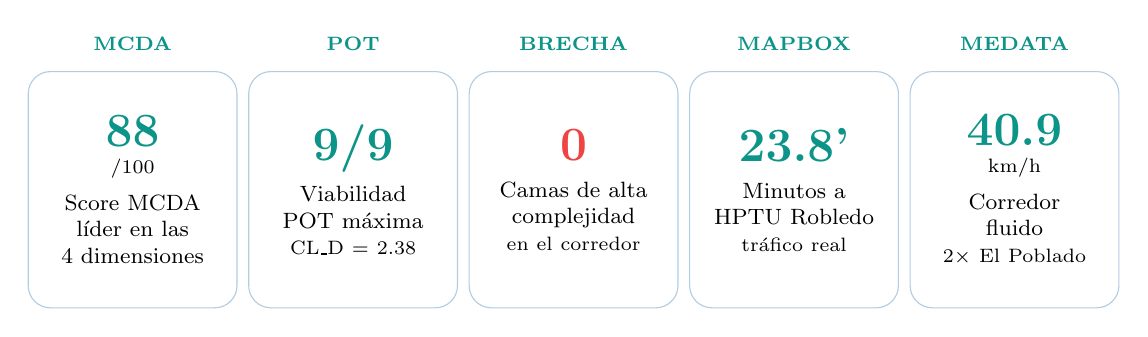
\begin{tikzpicture}[
  pillar/.style={draw=hptu!30, fill=white, rounded corners=8pt,
                 text width=2.3cm, minimum height=3.0cm, align=center,
                 font=\footnotesize, inner sep=5pt},
  plabel/.style={font=\scriptsize\bfseries, teal},
]
\node[pillar] (p1) at (0,0) {
  {\LARGE\textcolor{teal}{\textbf{88}}}\\{\scriptsize /100}\\[4pt]
  Score MCDA\\líder en las\\4 dimensiones
};
\node[pillar] (p2) at (2.8,0) {
  {\LARGE\textcolor{teal}{\textbf{9/9}}}\\[4pt]
  Viabilidad\\POT máxima\\{\scriptsize CL\_D = 2.38}
};
\node[pillar] (p3) at (5.6,0) {
  {\LARGE\textcolor{coral}{\textbf{0}}}\\[4pt]
  Camas de alta\\complejidad\\{\scriptsize en el corredor}
};
\node[pillar] (p4) at (8.4,0) {
  {\LARGE\textcolor{teal}{\textbf{23.8'}}}\\[4pt]
  Minutos a\\HPTU Robledo\\{\scriptsize tráfico real}
};
\node[pillar] (p5) at (11.2,0) {
  {\LARGE\textcolor{teal}{\textbf{40.9}}}\\{\scriptsize km/h}\\[4pt]
  Corredor\\fluido\\{\scriptsize 2$\times$ El Poblado}
};

\node[plabel, above=4pt of p1] {MCDA};
\node[plabel, above=4pt of p2] {POT};
\node[plabel, above=4pt of p3] {BRECHA};
\node[plabel, above=4pt of p4] {MAPBOX};
\node[plabel, above=4pt of p5] {MEDATA};
\end{tikzpicture}
\end{center}

\vspace{14pt}
\begin{center}
{\small Cinco líneas de análisis independientes ---MCDA, normativa, brecha hospitalaria, movilidad real y tráfico--- señalan la misma zona. Esa convergencia es lo que le da robustez a la recomendación preliminar.}
\end{center}
\end{frame}
}

% ============================================================
% SLIDE 16 — LA ZONA RECOMENDADA EN DETALLE
% ============================================================
\begin{frame}{La zona recomendada en detalle}

\begin{columns}[T]
\column{0.48\textwidth}
{\small\textbf{Ubicación}: Altos del Poblado / El Tesoro}\\
{\scriptsize Las Palmas Bajo: San Diego $\rightarrow$ La Colegiatura}

\vspace{4pt}
\begin{block}{\small Ficha técnica}
\scriptsize
\begin{tabular}{@{}p{3.4cm}l@{}}
\toprule
\textbf{Parámetro} & \textbf{Valor} \\
\midrule
Elevación & $\sim$1,700 msnm \\
Predios E5/E6 Comuna 14 & \highlight{38,415} \\
Avalúo promedio zona & \$245M COP \\
POT: carga dotacional & 2.38 (CL\_D) \\
Suelo potencial disponible & 68,020 m² \\
Altura máxima POT & 11.7 pisos \\
A Cl.\ Las Vegas / Milla de Oro & 10.5--10.7 min \\
A HPTU Robledo & 23.8 min \\
Competidores alta complejidad & \danger{0} \\
\bottomrule
\end{tabular}
\end{block}

\column{0.48\textwidth}
\vspace{2pt}
\begin{exampleblock}{\small ¿Por qué esta zona y no otra?}
\scriptsize
Es la \textbf{única zona} que combina simultáneamente:

\vspace{2pt}
\begin{enumerate}\setlength{\itemsep}{0pt}
  \item Demanda masiva a menos de 15 min
  \item Corredor vial que \textbf{fluye} en hora pico
  \item Viabilidad POT \textbf{máxima} para uso dotacional
  \item \textbf{Cero competencia} de alta complejidad
  \item VPN positivo en modelo financiero preliminar
\end{enumerate}
\end{exampleblock}

\vspace{2pt}
\begin{block}{\small Referencia sectorial}
\scriptsize El modelo de \textbf{San Vicente Rionegro} mostró que acercar la alta complejidad a la población objetivo puede funcionar. Las Palmas Bajo sigue esa lógica: llevar el HPTU al mercado E5/E6.
\end{block}
\end{columns}
\end{frame}

% ============================================================
% SLIDE 17 — LA PLATAFORMA INTERACTIVA (NUEVO)
% ============================================================
{
\setbeamercolor{background canvas}{bg=hptu!3}
\begin{frame}{La plataforma: 12 capas interactivas en tiempo real}

{\small Todo el análisis está disponible en una plataforma web interactiva, en vivo, con datos reales: {\textcolor{hptu}{\url{https://hptu-localizacion.vercel.app}}}}

\vspace{4pt}
\begin{columns}[T]
\column{0.48\textwidth}

\begin{block}{\small Capas del mapa interactivo}
\scriptsize
\begin{tabular}{@{}cl@{}}
\toprule
\textbf{\#} & \textbf{Capa} \\
\midrule
1 & Red de salud (145 IPS por complejidad) \\
2 & Densidad catastral E5/E6 \\
3 & Viabilidad POT (22 barrios) \\
4 & Segmentos de tráfico (velocidades) \\
5 & Isocronas por zona candidata \\
6 & Corredor Las Palmas (límite) \\
7 & Rutas alternativas validadas \\
8 & POIs: colegios, clubes, corporativo \\
9 & Zonas de estrato (ArcGIS) \\
10 & Lotes potenciales de desarrollo \\
11 & Red hospitalaria completa (1,536) \\
12 & Zonas candidatas (5) con scores \\
\bottomrule
\end{tabular}
\end{block}

\column{0.48\textwidth}
\begin{exampleblock}{\small 17 secciones de análisis}
\scriptsize
\begin{itemize}\setlength{\itemsep}{0pt}
  \item Mapa interactivo con filtros por capa
  \item Gradiente de demanda (timeline visual)
  \item Gráficos de velocidad y volumen vehicular
  \item Brecha hospitalaria (barras + tabla)
  \item Radar MCDA comparativo (5 zonas)
  \item Modelo financiero por zona
  \item Análisis DENSURBAM (IRS + proyecciones)
  \item Arquitectura de datos y fuentes
  \item Cronograma y entregables
\end{itemize}
\end{exampleblock}

\vspace{1pt}
{\scriptsize\textbf{Stack}: Next.js 14 · Mapbox GL · Recharts · TypeScript · 15 GeoJSON · Datos reales · Vercel}
\end{columns}
\end{frame}
}

% ============================================================
% SLIDE 18 — MODELO FINANCIERO
% ============================================================
\begin{frame}{Modelo financiero preliminar}

{\footnotesize\textcolor{slate}{Estas cifras son una \textbf{primera aproximación}. Los parámetros con {\textcolor{coral}{$\blacktriangledown$}} requieren validación con el sector.}}

\vspace{4pt}
\begin{columns}[T]
\column{0.54\textwidth}

{\scriptsize
\begin{tabular}{@{}l r r r r@{}}
\toprule
\textbf{Zona} & \textbf{Camas} & \textbf{Inversión} & \textbf{Payback} & \textbf{VPN 10y} \\
\midrule
\rowcolor{teal!10}
\textbf{LP Bajo} & \textbf{250} & \textbf{\$90MM} & \textbf{11.3y} & \highlight{+\$4.8MM} \\
LP Medio & 300 & \$108MM & 9.4y & +\$15.3MM \\
Envigado & 220 & \$82MM & 11.3y & +\$4.0MM \\
N.\ Poblado & 260 & \$98MM & 9.6y & +\$14.7MM \\
\rowcolor{coral!8}
LP Alto & 150 & \$55MM & \danger{22.9y} & \danger{--\$31MM} \\
\bottomrule
\end{tabular}
}
{\tiny Cifras en miles de millones COP. WACC 12\%, ramp-up 60\%/80\%/100\% en años 1/2/3+.}

\vspace{4pt}
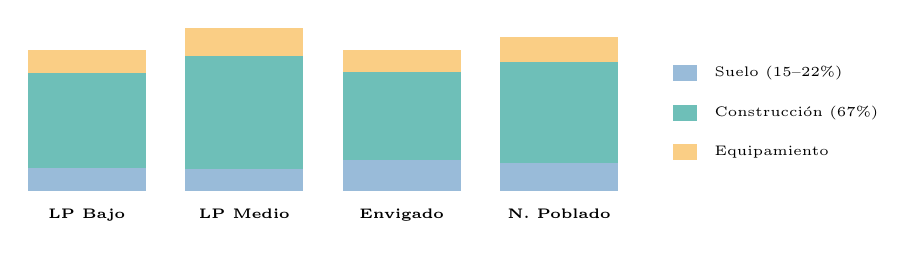
\begin{tikzpicture}
  \foreach \x/\label/\land/\const/\equip in {
    0/LP Bajo/15/60/15,
    2/LP Medio/14/72/18,
    4/Envigado/20/56/14,
    6/N. Poblado/18/64/16} {
    \pgfmathsetmacro{\landh}{\land/90*1.8}
    \pgfmathsetmacro{\consth}{\const/90*1.8}
    \pgfmathsetmacro{\equiph}{\equip/90*1.8}
    \fill[hptu!40] (\x,0) rectangle (\x+1.5, \landh);
    \fill[teal!60] (\x,\landh) rectangle (\x+1.5, \landh+\consth);
    \fill[amber!50] (\x,\landh+\consth) rectangle (\x+1.5, \landh+\consth+\equiph);
    \node[font=\tiny\bfseries, below] at (\x+0.75, -0.1) {\label};
  }
  \fill[hptu!40] (8.2,1.4) rectangle (8.5,1.6); \node[font=\tiny, right] at (8.6,1.5) {Suelo (15--22\%)};
  \fill[teal!60] (8.2,0.9) rectangle (8.5,1.1); \node[font=\tiny, right] at (8.6,1.0) {Construcción (67\%)};
  \fill[amber!50] (8.2,0.4) rectangle (8.5,0.6); \node[font=\tiny, right] at (8.6,0.5) {Equipamiento};
\end{tikzpicture}

\column{0.43\textwidth}
\begin{block}{\small Parámetros base}
\scriptsize
\begin{tabular}{@{}ll@{}}
Construcción/m² & \$4.0M {\tiny(Scielo/U.\ Mil.)} \\
Dotación & 25\% {\tiny(DNP)} \\
Ocupación & 80\% \\
Ingreso/cama/año & \$1,600M {\tiny(HUSI)} {\color{coral}$\blacktriangledown$} \\
EBITDA & 8\% {\color{coral}$\blacktriangledown$} \\
WACC & 12\% {\color{coral}$\blacktriangledown$} \\
Timeline total & 54 meses (4.5 años) \\
\end{tabular}
\end{block}

\vspace{2pt}
\begin{exampleblock}{\small Hallazgo clave}
\scriptsize El suelo representa solo el \textbf{15--22\%} del costo total. Lo que importa es el tamaño del lote y la altura del POT, no el precio entre zonas.
\end{exampleblock}

\vspace{1pt}
{\scriptsize\textcolor{slate}{4 de 5 zonas con VPN positivo. LP Alto es la única inviable.}}
\end{columns}
\end{frame}

% ============================================================
% SLIDE 19 — SENSIBILIDAD Y SUPUESTOS
% ============================================================
{
\setbeamercolor{background canvas}{bg=amber!4}
\begin{frame}{Sensibilidad del modelo y supuestos por validar}

\begin{columns}[T]
\column{0.48\textwidth}
\begin{alertblock}{\small El parámetro más sensible}
\scriptsize El ingreso por cama/año determina la viabilidad:

\vspace{3pt}
{\scriptsize
\begin{tabular}{@{}lrr@{}}
\toprule
\textbf{Escenario} & \textbf{Ingreso/cama} & \textbf{VPN LP Bajo} \\
\midrule
\rowcolor{coral!6}
Conservador (HUSI) & \$1,600M & +\$4.8MM \\
\rowcolor{teal!6}
Privado premium & \$2,000M & \highlight{+\$25MM} \\
Privado alto & \$2,200M & +\$38MM \\
\bottomrule
\end{tabular}
}

\vspace{3pt}
{\scriptsize Un cambio de +25\% en ingreso/cama multiplica el VPN \textbf{5 veces}. Es el primer parámetro que necesitamos validar.}
\end{alertblock}

\vspace{3pt}
\begin{block}{\small Riesgos identificados}
\scriptsize
\begin{enumerate}\setlength{\itemsep}{0pt}
  \item Demoras en licenciamiento POT
  \item Volatilidad costos de construcción
  \item Cartera EPS ($\sim$\$14B COP en el sector)
  \item Nuevos competidores en el corredor
  \item Cambios regulatorios (POT / salud)
\end{enumerate}
\end{block}

\column{0.48\textwidth}
\begin{alertblock}{\small Supuestos por validar}
\scriptsize
\begin{tabular}{@{}p{2.8cm}cc@{}}
\toprule
\textbf{Parámetro} & \textbf{Prior.} & \textbf{Fuente} \\
\midrule
\rowcolor{coral!8}
Precio suelo/m² & \danger{Alta} & Lonja \\
\rowcolor{coral!8}
Ingreso/cama/año & \danger{Alta} & HPTU \\
\rowcolor{coral!6}
Margen EBITDA & \danger{Alta} & Supersalud \\
Fichas POT polígono & \danger{Alta} & DAP Med. \\
Lotes disponibles & \danger{Alta} & Inmobil. \\
\rowcolor{amber!10}
WACC proyecto & Media & Banca inv. \\
\rowcolor{amber!10}
Costos licencias & Media & Arq.\ hosp. \\
\bottomrule
\end{tabular}
\end{alertblock}

\vspace{3pt}
\begin{exampleblock}{\small Lectura ejecutiva}
\scriptsize La \textbf{dirección} de la recomendación (Las Palmas Bajo) se sostiene con datos sólidos. La \textbf{magnitud} de la inversión depende de validar estos 7 supuestos. Ese es el trabajo de la Fase 3.
\end{exampleblock}
\end{columns}
\end{frame}
}

% ============================================================
% SLIDE 20 — ESTADO DEL ESTUDIO
% ============================================================
\begin{frame}{Transparencia: qué hemos construido y qué falta}

\begin{columns}[T]
\column{0.48\textwidth}
\begin{exampleblock}{\small Lo que ya está construido (sólido)}
\scriptsize
\begin{enumerate}\setlength{\itemsep}{1pt}
  \item[\textcolor{teal}{\checkmark}] \textbf{Demanda georreferenciada}: 174,543 predios E5/E6 en 22 barrios, con avalúos del Catastro
  \item[\textcolor{teal}{\checkmark}] \textbf{Brecha hospitalaria}: 145 IPS mapeadas, 0 camas alta complejidad en el corredor
  \item[\textcolor{teal}{\checkmark}] \textbf{Movilidad real}: 682,502 obs.\ + tiempos Mapbox + validación Google Routes
  \item[\textcolor{teal}{\checkmark}] \textbf{Viabilidad POT}: 22 barrios con score, CL\_D, altura, suelo potencial
  \item[\textcolor{teal}{\checkmark}] \textbf{Modelo MCDA}: 5 zonas, 4 dimensiones, ranking robusto
  \item[\textcolor{teal}{\checkmark}] \textbf{Plataforma interactiva}: 12 capas, mapa en vivo, trazabilidad completa
\end{enumerate}
\end{exampleblock}

\column{0.48\textwidth}
\begin{alertblock}{\small Lo que falta por validar (en construcción)}
\scriptsize
\begin{enumerate}\setlength{\itemsep}{1pt}
  \item[\textcolor{coral}{$\blacktriangledown$}] \textbf{Precio suelo/m²} por zona\\
    {\tiny Fuente: Lonja de Propiedad Raíz}
  \item[\textcolor{coral}{$\blacktriangledown$}] \textbf{Ingreso/cama/año} alta complejidad\\
    {\tiny Fuente: HPTU, Cl.\ Las Américas, Supersalud}
  \item[\textcolor{coral}{$\blacktriangledown$}] \textbf{Margen EBITDA} operativo real\\
    {\tiny Fuente: Supersalud, estados financieros}
  \item[\textcolor{coral}{$\blacktriangledown$}] \textbf{Fichas normativas POT} por polígono\\
    {\tiny Fuente: DAP Medellín}
  \item[\textcolor{coral}{$\blacktriangledown$}] \textbf{Lotes disponibles} con propietarios\\
    {\tiny Fuente: inmobiliarias del corredor}
  \item[\textcolor{amber}{$\blacktriangledown$}] \textbf{WACC específico} del proyecto\\
    {\tiny Fuente: banca de inversión}
\end{enumerate}
\end{alertblock}
\end{columns}

\vspace{4pt}
\begin{center}
{\small Lo que tenemos hoy es suficiente para \textbf{definir la dirección}. La decisión de inversión requiere completar la Fase 3.}
\end{center}
\end{frame}

% ============================================================
% SLIDE 21 — QUÉ SIGUE
% ============================================================
\begin{frame}{Qué sigue y qué necesitamos de ustedes}

\begin{columns}[T]
\column{0.50\textwidth}
{\small\textbf{Fase 3 — Profundización} (en curso)}

\vspace{3pt}
\begin{enumerate}\scriptsize
  \setlength{\itemsep}{1pt}
  \item[\textcolor{teal}{\textbf{1.}}] \textbf{Validar modelo financiero} con datos reales del sector
  \item[\textcolor{teal}{\textbf{2.}}] \textbf{Due diligence normativo}: fichas POT por polígono
  \item[\textcolor{teal}{\textbf{3.}}] \textbf{Identificar 2--3 lotes} concretos con inmobiliarias
  \item[\textcolor{teal}{\textbf{4.}}] \textbf{Análisis de sensibilidad} robusto (escenarios)
  \item[\textcolor{teal}{\textbf{5.}}] \textbf{Competencia detallada}: servicios, tarifas, especialidades
\end{enumerate}

\vspace{4pt}
{\small\textbf{Fase 4 — Recomendación Final}}\\
{\scriptsize Informe ejecutivo · Shortlist de lotes · Escenarios de inversión · Presentación a Junta Directiva}

\vspace{4pt}
{\scriptsize\textbf{Entregables del estudio completo:} Plataforma web (12 capas) · Informe técnico PDF · Base georreferenciada (GeoJSON) · Modelo financiero con sensibilidad · Presentación final para Junta.}

\column{0.47\textwidth}
\begin{alertblock}{\small Lo que necesitamos de ustedes}
\scriptsize Para avanzar en la Fase 3, necesitamos acceso o contacto con:

\vspace{3pt}
\begin{enumerate}\setlength{\itemsep}{1pt}
  \item[\textcolor{coral}{\textbf{1.}}] \textbf{Lonja de Propiedad Raíz}\\
    {\tiny Precios reales de suelo por zona}
  \item[\textcolor{coral}{\textbf{2.}}] \textbf{Datos financieros HPTU}\\
    {\tiny Ingreso/cama, EBITDA, ocupación real}
  \item[\textcolor{coral}{\textbf{3.}}] \textbf{DAP Medellín}\\
    {\tiny Fichas normativas POT del corredor}
  \item[\textcolor{amber}{\textbf{4.}}] \textbf{Inmobiliarias / corredores}\\
    {\tiny Lotes disponibles en la zona}
  \item[\textcolor{amber}{\textbf{5.}}] \textbf{Supersalud}\\
    {\tiny Márgenes operativos del sector}
\end{enumerate}
\end{alertblock}
\end{columns}
\end{frame}

% ============================================================
% SLIDE 22 — CIERRE
% ============================================================
{
\setbeamercolor{background canvas}{bg=hptu}
\begin{frame}[plain]
\vfill
\begin{center}

{\large\textcolor{white!90}{Un hospital saturado al 96\%.}}

\vspace{4pt}
{\large\textcolor{white!90}{Un corredor con 174,543 predios E5/E6.}}

\vspace{4pt}
{\large\textcolor{white!90}{Y cero camas de alta complejidad.}}

\vspace{20pt}
\begin{tikzpicture}
  \draw[white, line width=0.5pt] (0,0) -- (8,0);
\end{tikzpicture}

\vspace{18pt}
{\Large\bfseries\textcolor{white}{Los datos convergen.\\[4pt]
Seguimos construyendo la evidencia.}}

\vspace{20pt}
{\small\textcolor{white!70}{Plataforma interactiva:}}\\
{\small\textcolor{white!90}{\url{https://hptu-localizacion.vercel.app}}}

\vspace{10pt}
{\small\textcolor{white!50}{15 fuentes oficiales · 3.8M+ registros · 12 capas · 5 zonas · Modelo MCDA}}

\vspace{16pt}
{\footnotesize\textcolor{white!40}{6 de marzo, 2026 · Fourier.dev}}
\end{center}
\vfill
\end{frame}
}

\end{document}
